\section {MEMS (Mikro-Elektro-Mechanische-Systeme)}
\begin{compactitem}
    \item Materialen: Silizium, Polymere, Metalle, Keramik
\end{compactitem}


\subsection{Herstellungsverfahren}
\subsubsection{Bulk Micromachining}
\begin{multicols}{2}
    \begin{compactitem}
      \item Selektives Ätzen aus dem Silizium
      \item Ätzmittel: Fluorwasserstoff, Salpetersäure, Essigsäure (korrosiv)
      \item Vorteile:
      \begin{compactitem}
          \item Schnelles, gleichförmiges Verfahren über grosse Waferflächen
          \item Günstig bezüglich Zeit & Geld
      \end{compactitem}
      \item Nachteile:
      \begin{compactitem}
          \item Keine komplexen Strukturen
          \item Nicht geeignet für Submikrometerbereich (Undercut)
      \end{compactitem}
      \item Anwendung:
      \begin{compactitem}
          \item Drucksensoren
      \end{compactitem}
    \end{compactitem}

    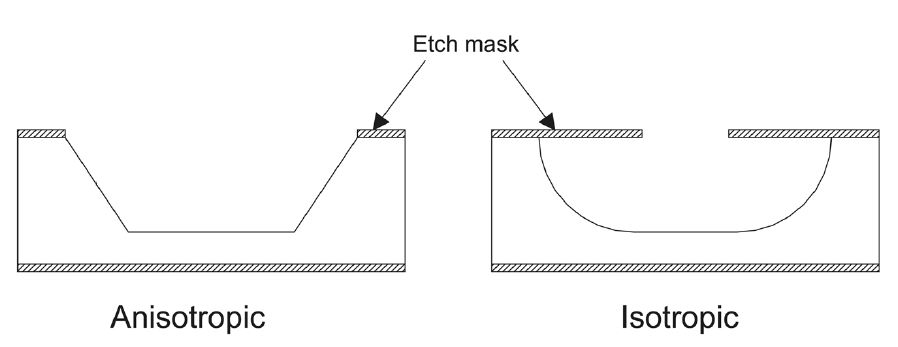
\includegraphics[width=0.54\textwidth]{images/Bulk_Micro}
\end{multicols}



\subsubsection{Surface Micromachining}
	\begin{minipage}{0.4\textwidth}
      \begin{compactitem}
        \item Schichtenaufbau mit Ätzen:
        \begin{compactitem}
            \item Siliziumnitrid $\rightarrow$ Schützt Substrat
            \item Siliziumoxid $\rightarrow$ Opferschicht
            \item Maske auf Siliziumoxid
            \item Polysilizium  $\rightarro$ Tragende Schicht
            \item Wegätzen der Opferschicht
            \item (Ähnlich IC-Produktion)
        \end{compactitem}
      \end{compactitem}

	  \begin{compactitem}
	    \item Schichtenaufbau mittels Sputtering:
        \begin{compactitem}
            \item Wafer in Vakuumkammer an Anode
            \item Opfermaterial (bspw. Metall) an Kathode
            \item Ionisiertes Gas (Argon) einleiten
            \item Gasionen treffen auf Opfermaterial
            \item Metallatome haften auf Wafer
        \end{compactitem}
      \end{compactitem}  
      \begin{compactitem}
        \item Vorteile:
        \begin{compactitem}
          \item AnisotropischesVerfahren $\rightarrow$ Keine Undercuts
          \item Komplexere Strukturen
        \end{compactitem}
        \item Nachteile:
          \begin{compactitem}
            \item Sputtering $\rightarrow$ Strahlungsschäden
            \item Zeitaufwändiger und teurer
          \end{compactitem}
      \end{compactitem}
    \end{minipage}
    \hfill
    \begin{minipage}{0.5\textwidth}
    \vspace{-0pt}
      \begin{compactitem}
       \item Anwendung:
        \begin{compactitem}
          \item Freiträger, Brücken, Hohlräume
          \item Turbinen, Zahnräder
        \end{compactitem}
      \end{compactitem}
      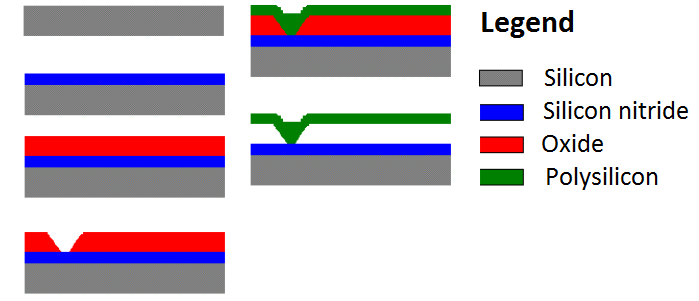
\includegraphics[width=1\textwidth]{images/Schichtenaufbau}
      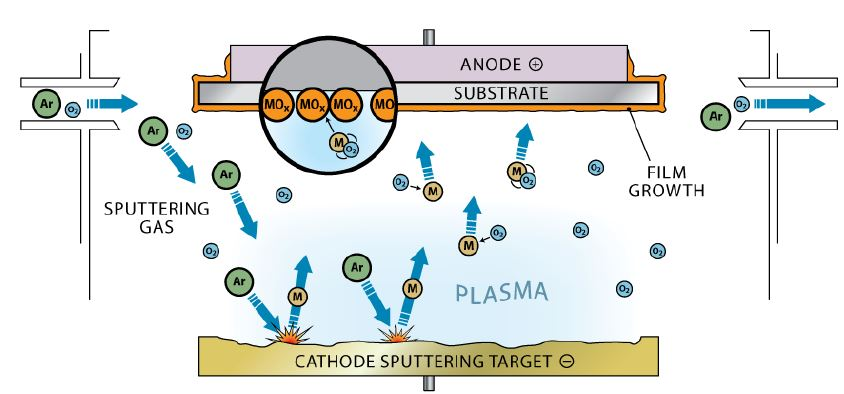
\includegraphics[width=1.\textwidth]{images/Sputtering}
	\end{minipage}


\subsection{MEMS Oszillatoren}
	\begin{minipage}{0.4\textwidth}
      \begin{compactitem}
        \item Vorteile:
        \begin{compactitem}
          \item FlexibeleinstellbareFrequenz
          \item Low cost
        \end{compactitem}
        \item Nachteile:
        \begin{compactitem}
          \item Toleranzen sind gross (ca. 10\%) $\rightarrow$ Abgleich nötig $\rightarrow$ PLL 
        \end{compactitem}
         \item Anwendungsfrequenz: 1Hz - 625 MHz bis 6 decimals (ppm)
      \end{compactitem}
    \end{minipage}
    \hfill
    \begin{minipage}{0.5\textwidth}
       \vspace{0pt}
       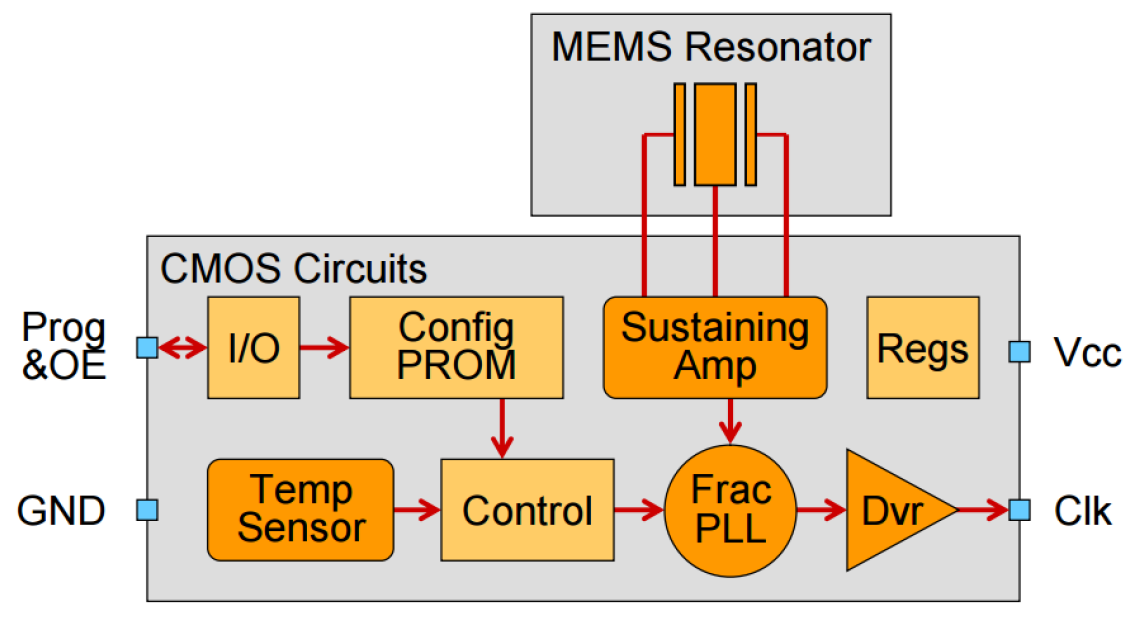
\includegraphics[width=0.9\textwidth]{images/MEMS_Oszillator}   
    \end{minipage}


\subsection{Grundformeln}
\label{subsec:Grundformeln}
\subsubsection{Mechanik}
	\begin{minipage}{0.3\textwidth}
      \begin{equation*} 
        \begin{split} 
            &\overrightarrow{F}=\overrightarrow{a} \cdot m\\
            &F=k_m \cdot \Delta x  \quad (\text{Federkonstante } K_m)\\
            &\Delta x=\frac{m}{k_m} \cdot a\\
            &F_d \sim \frac{d_x}{dt} \quad (\text{Dämpfungskraft } F_d)\\
            &F(t)=m\cdot \frac{d^2}{dt^2}x(t)+D \cdot \frac{d}{dt}x(t)+k_m \cdot x(t)\\
            &F(s)=(m \cdot s^2 + D \cdot s + k_m)\cdot X(s) \\
            &H{sensor}(s)=\frac{X(s)}{F(s)}=\frac{1}{m\cdot s^2 + D\cdot s + k_m} \\
            &\text{D: Dämpfungskonstante}
        \end{split} 
      \end{equation*}
    \end{minipage}
    \hfill
    \begin{minipage}{0.6\textwidth}
      \vspace{0pt}
      \paragraph{Verglich mit TP 2.Ordnungm}
      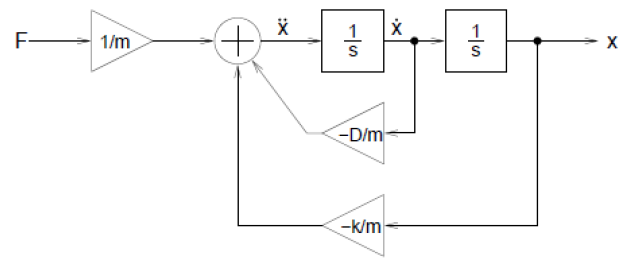
\includegraphics[width=1.0\textwidth]{images/Mech_Regel}  
    
      \begin{minipage}{1.0\textwidth}
        \vspace{0pt}
        \hspace{1cm}
        $\omega _0= \sqrt{\frac{k_m}{m}}$   $ \quad \quad Q=\frac{m\cdot  \omega_0}{D}$
        $\quad \quad H_{LP}= \frac{A \cdot \omega_0 ^2}{s^2 +\frac{\omega _0=}{Q}\cdot s + \omega _0 ^2}$
       \end{minipage}
    \end{minipage}
    
\subsubsection{Elektrostatik}

    $C=\frac{Q}{V} \quad \quad \quad E=\frac{1}{2}\cdot C \cdot V^2 \quad \quad \quad F_{es}=\frac{d}{d_x}\cdot E = \frac{1}{2} \cdot \frac{d}{d_x} \cdot C \cdot V^2$
    
\paragraph{Für parallele Platten}
    \begin{minipage}{0.4\textwidth}
    \vspace{-1cm}
    \begin{equation*} 
      \begin{split} 
         &C(x)=\frac{\epsilon_r \cdot \epsilon_0 \cdot A}{x_0 + x} \\
         &F_{es}(x)=\frac{\epsilon_r \cdot \epsilon_0 \cdot A}{2(x_0+x)^2}\cdot V^2 \approx -\frac{A\epsilon_0\epsilon_r V^2}{2x_0^2}+\frac{A\epsilon_0\epsilon_r V^2}{x_0^3}\cdot x 
      \end{split} 
    \end{equation*}
    \end{minipage}
    \hfill
    \begin{minipage}{0.4\textwidth}
      \vspace{0pt}
      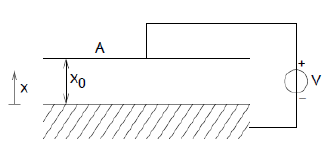
\includegraphics[width=0.9\textwidth]{images/Plattenkondens}
    \end{minipage}

\vspace{-0.5cm}
\subsubsection{Elektrostatische Federkonstante}
\vspace{-0.5cm}
    \begin{equation*} 
      \begin{split} 
        &F(t)=m\cdot \frac{d^2}{dt^2}x(t)+D \cdot \frac{d}{dt}x(t)+(k_m- \frac{A\epsilon_0\epsilon_r V^2}{x_0^3})x(t)= -\frac{A\epsilon_0\epsilon_r V^2}{2x_0^2}+F \\
        &k_{eff}=k_m+k_{es}=k_m- \frac{A\epsilon_0\epsilon_r V^2}{x_0^3} \quad \quad \text{(}k_{eff} \quad \text{darf nicht negativ werden und beeinflusst Resonanzfrequenz.)}\\
      \end{split} 
    \end{equation*}

\subsection{Messung Auslenkung}
\begin{minipage}{0.6\textwidth}
  Kleine Auslenkungen können mit zwei Kondensatorplatten gemessen werden (siehe \ref{subsec:Grundformeln}). Für grössere Auslenkungen kann ein System mit konstanter Lasung $Q$ verwendet werden (Charge control). Gesamte Energie im System: \\
    \begin{equation*} 
        \begin{split} 
           &E=\frac{Q^2}{2C}=\frac{(x_0 + x)Q^2}{2A\epsilon_0 \epsilon_r}
        \end{split} 
    \end{equation*}
  Für 2 C: keine Kraft wirkt, wenn kein Strom durch $mid$ fliesst.\\ $\rightarrow$ Spannungsmessung, nicht Ladungsverstärker.
\end{minipage}
\begin{minipage}{0.3\textwidth}
    \vspace{0pt}
    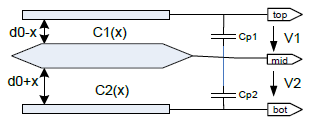
\includegraphics[width=1.2\textwidth]{images/Bewegung_C}
\end{minipage}
\begin{compactitem}
    \item Vorteile: Einfaches Syste
\end{compactitem}
\begin{compactitem}
    \item Nachteile: Auslenkund ist nichtlineare Funktion der Kraft, Messung mit Ladungsverstärkter bewirkt ebenfalls Kraft
\end{compactitem}


\subsubsection{Kamm-Struktur für grössere Auslenkungen, z.B. Gyros}
\begin{minipage}{0.3\textwidth}
\vspace{-0.5cm}
  \begin{equation*}
    \begin{split} 
      &h\text{:       Dicke der Struktur}\\
      &n_{gap}\text{: Anzahl Abstände}\\
      &g\text{:       Abstand}\\
    \end{split} 
  \end{equation*}
\end{minipage}
\begin{minipage}{0.3\textwidth}
\vspace{-0.5cm}
  \begin{equation*} 
    \begin{split} 
      &C=\frac{\epsilon_0 \epsilon_r\cdot n_{gap}(x_0-x)h}{g}\\
      &E=\frac{1}{2}CV^2\\
      &F_{es}=-\frac{\epsilon_0 \epsilon_r \cdot n_{gap} h v^2}{2g}\\
    \end{split} 
  \end{equation*}
\end{minipage}
\begin{minipage}{0.3\textwidth}
    \vspace{-0.7cm}
    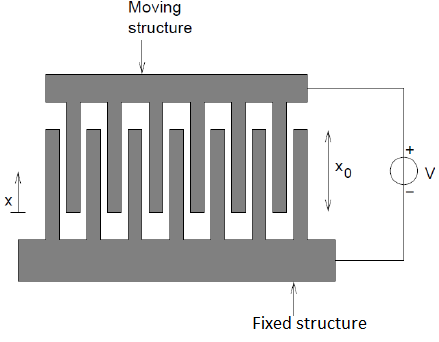
\includegraphics[width=1.2\textwidth]{images/Kamm_Strukt}
\end{minipage}

\vspace{-0.5cm}
\subsection{Messung mit Force Feedback}
\begin{minipage}{0.4\textwidth}
  \begin{compactitem}
    \item Ziel: 
    \begin{compactitem}
        \item Masse in Mitte halten
        \item elektrostat. Kraft als Gegenkraft zur mech. Kraft  aufbringen
        \item elektrostat. Kraft wird kontrolliert, ist bekannt $\rightarrow$ Beschleunigung kann berechnet werden.
    \end{compactitem}
  \end{compactitem}
  \begin{compactitem}
    \item Vorteile:  Elektrostatische Kraft ist bekannt $(F\simV)$, linear
  \end{compactitem}
  \begin{compactitem}
    \item Nachteile: Regelkreis kann instabil werden bei hoher Ordnung
  \end{compactitem}
\end{minipage}
\hfill
\begin{minipage}{0.5\textwidth}
    \vspace{0pt}
    \hspace{-0.7cm}
    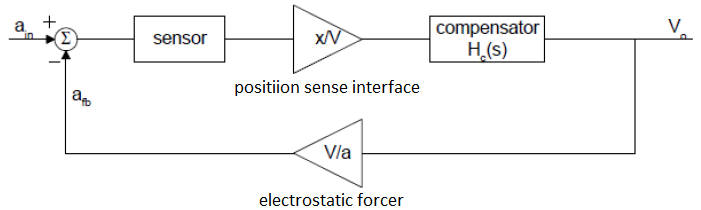
\includegraphics[width=1.1\textwidth]{images/Force_Feedback}
\end{minipage}

\subsection{Auswertung von Kapazitäten}
\subsubsection{Auswertung mit Demodulation}
\begin{minipage}{0.3\textwidth}
  Die beiden Kondensatoren werden mit inversen Rechteck-Impulsen angesteuert. Am Ausgang des Verstärkers erhält man dann immer einmal ein pos. und sonst ein neg. Signal. Dieses wird dann mit $\pm 1$ muliipliziert, um ein positives Signal zu erhalten, welches dann noch gefiltert wird, bevor es dann auf einen ADC geht.
\end{minipage}
\hfill
\begin{minipage}{0.6\textwidth}
    \vspace{0pt}
    \hspace{-0.7cm}
    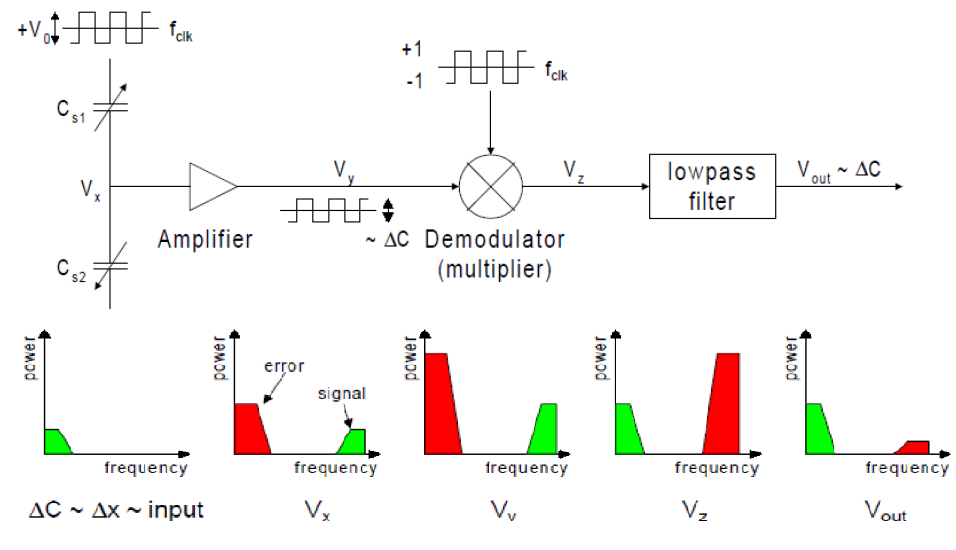
\includegraphics[width=1.0\textwidth]{images/Demodulation}
\end{minipage}

\subsubsection{Ladungsverschiebung und Charge Sensing}
 $V_{out}$ lässt sich für beide gleich berechnen:   $V_{out}=-V_0 \cdot \frac{\Delta C }{C_{int}}\quad \quad \quad C_{int} \approx 2C_0$  (typisch, Gain-Speed Tradeoff)   \\
Nachteil: Elektrostatische Kräfte beeinflussen mech. Verhalten.\\
Vorteil bei Charge-Sensing: Paracitics werden nicht umgeladen, haben daher keinen Einfluss auf Ausgangssignal.
\hfill
\begin{minipage}{0.45\textwidth}
    \vspace{0pt}
    \hspace{-0.7cm}
    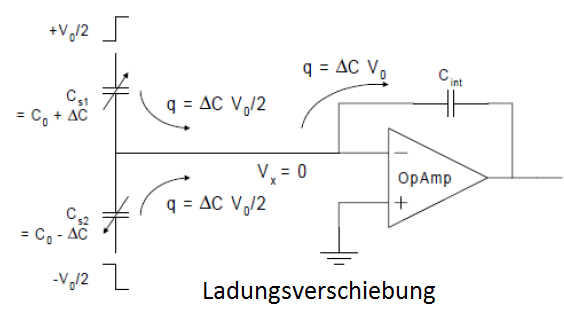
\includegraphics[width=1.0\textwidth]{images/Ladungsverschiebung}
\end{minipage}
\hfill
\begin{minipage}{0.45\textwidth}
    \vspace{0pt}
    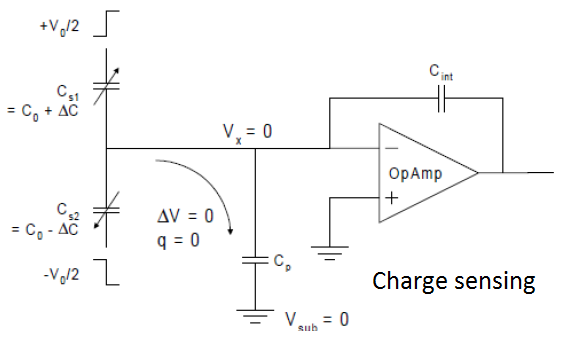
\includegraphics[width=1.0\textwidth]{images/charge_sensing}
\end{minipage}

\section{Konstanten}
$k = 1,3806505 \cdot 10^{-23} J/K$ \ \ \ \ \ \ \ \ \ \ $\epsilon_0 = 8.8541...\cdot 10^{-12} \frac{As}{Vm}$ \\
$T$ in Kelvin: 273,15 +  $\vartheta$  in °C \ \ \ \ \ \
$\mu _0 = 4\pi \cdot 10^{-7} \frac{N}{A^2}=1.2566..\cdot 10^{-7} \frac{N}{A^2}

